\section{GIF}

\subsection{Aperçu du GIF}
Le format GIF permet de stocker plusieurs images dans un fichier. 
Ceci permet de créer des diaporamas, voire des animations si les images sont affichées à un rythme suffisamment soutenu. 
Chaque image d'une animation peut avoir sa propre palette.
Le GIF est un format très utilisé, particulièrement sur les réseaux sociaux. 
Ce projet peut donc intéressé pas mal de gens.\\
La structure du format GIF est connue et disponible en ligne. En voici un schéma : 

\vspace{1.5cm}
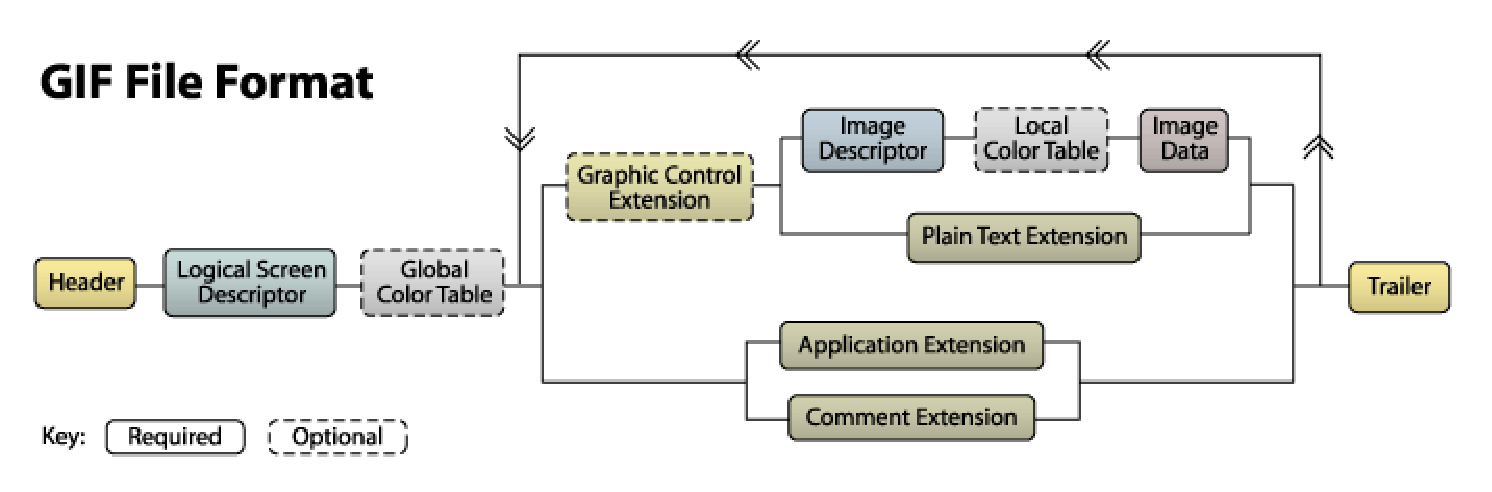
\includegraphics[width=15cm]{gif_structure.eps}

\vspace{1.5cm}
\subsection{Application du LSB}
Nous avons choisi de cacher des informations dans les bytes des Local Color Table. 
Les Color Table décrivent des couleurs, chaque couleur étant codée sur 3 bytes. 
Ces informations ne sont pas compressées contrairement au bloc image data.\\

Cette section, Local Color Table, est facultative et peut revenir devant chaque bloc image data. 
Si elle n'existe pas, nous la rajoutons en copiant
alors la global color table.
Au final, on aura autant de local color table qu'il y a de blocs image data.\\

Il est possible de calculer la taille maximale du message cachée à l'avance. 
Pour cela, on compte le nombre de bytes que l'on peut cacher par Color Table : nombre de bytes dans une color Table / 8.
Puis, on multiplie cela par le nombre potentiel de Local Color Table dans le fichier, ce qui revient à compter le nombre de bloc image data.

\vspace{1.5cm}
